\section{Method}
The below described implementations have been trained ensuring that in every iteration the starting point is the same between two methods, in order to evaluate the two algorihtms in the exact same conditions.


\subsection{Reinforcement Learning}
The reinforcement learning implementation is based on temporal differenc learning \cite{sutton1998temporal}, 
in particular Q-learning.
The implementation takes inspiration from the work of \textit{JackFurby} \cite{JackFurbyCartPole}.

The \textit{Q-table} is represented by the discretization of the continuous 4-dimensional state vector in 20 even intervals for every dimension of the vector leading to 160000 possible pairs of $<state,action>$, considering the two possible actions, Figure \ref{figDISC} shows an example of the explained state-discretization.

\begin{figure}[H]
	\centering
	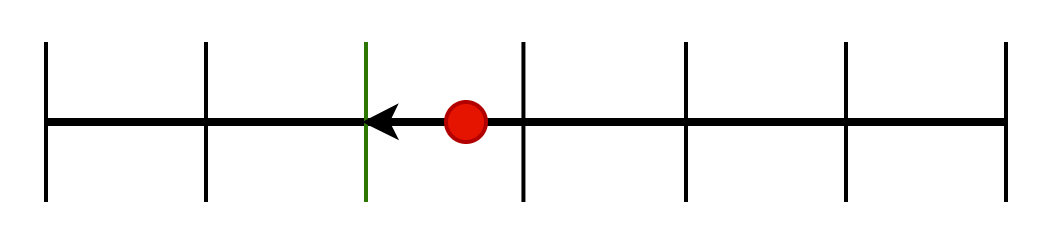
\includegraphics [scale = 0.2]{Images/state_discretization.png}
	\caption{Representation of the state discretization technique, considering an element of the state, $s_i$, the red dot is the real value of $s_i$, this is discretized to the nearest leftwise discrete state.}
	\label{figDISC}
\end{figure}

Once an action is performed, the state selected is the first larger that the observed state.\\
The parameters used in the experiments are the following:


\begin{table}[htb]%
	\centering
	\label{tab:RL_parameters}
	\begin{tabular}{|S|S|} 		% S = special column format from the siunitx package. Aligns commas.
		
		\hline
		{\textbf{Learning rate $\alpha$}} &  {0.1} \\
		\hline
		{\textbf{Discount factor $\gamma$}} & {1} \\
		\hline
		{\textbf{Number of episodes $n_{ep}$}} & {20000} \\
		\hline
		{\textbf{Exploration rate $\varepsilon$}}  & {decaying} \\
		\hline
		{\textbf{Penalty factor $PF$}}& {-375} \\
		\hline
		
	\end{tabular}
	\caption{Parameters used in the RL implementation. The exploration rate $\varepsilon$ starts with $\varepsilon(0)=1$ and decays by $\varepsilon(t) = \varepsilon(t - 1) - \frac{1}{\frac{n_{ep}}{2} - 1}$, every episode, stopping after $\frac{n_{ep}}{2}$ episodes. The penalty factor penalize the Q-value of the determinated state-action tuple of a value \textit{PF}}
\end{table}



\subsection{Genetic Algorithms}

\subsubsection{Genotype}
Since Genetic Algorithms can be very different depending on the genotype chosen to represent individuals, we have tried several different implementation of GA, varying the used genotype.
\\


The first method used is a very naive implementation that can be applied to a very large variety of problems with GA : reprensenting individuals with the vector of all actions they will perform in order.
Thus, \textit{i-th} character of the genotype of an individual $j$ corresponds to the \textit{i-th} action performed by the corresponding individual.
In this apporach, mutation is performed by switching an action in the genotype from left to right or from right to left with a probability given by the \textit{Mutation rate} for every action $i$ inside the genotype.
\\
Since this particular genotype does not generalize well with the random initialization of the starting position of the pole. Due its intrinisc dependecy with the initial state, fixed starting conditions should be applied to obtain good results with this genotype, forcing the environment to always start at the same place, but this leads to a scarse ability of generalization, since the training is valid just for a determinated starting position of the pole.

All those considerations lead to the decision of evaluating other encodings for the final implementation.\\

The second encoding takes inspiration from Reinforcement Learning \textit{Q-table}.
In this approach, the focus is not to predict every action individually  but instead use GA to assign values to state-actions pairs then select the action that referes to the observed state.\\
The discretization techninque mirrors that utilized in the reinforcement learning implementation and briefly outlined in Figure \ref{figDISC}.\\
Here, mutation is performed by swapping the action of a given state with a probability determined by the \textit{Mutation rate}.


\subsubsection{Parameters}
The GA parameters can be found in the following table :
\begin{table}[htb]%
	\centering
	\begin{tabular}{|S|S|} 		% S = special column format from the siunitx package. Aligns commas.
		
		\hline
		{\textbf{Genotype}} &  {Q-table} \\
		\hline
		{\textbf{Population Size}} & {100} \\
		\hline
		{\textbf{Generations}} & {200} \\
		\hline
		{\textbf{Selection}}  & {Fitness} \\
		\hline
		{\textbf{Mutation Rate}} & {0.005} \\
		\hline
		{\textbf{Crossover}}& {one-point} \\
		\hline
		{\textbf{Elitism}}&  {2}  \\
		\hline

	\end{tabular}
	\caption{Parameters used in the GA implementation, the \textit{Elitims} parameter describe how many individual from the last generation are saved for the successive one}
	\label{tab:GA_parameters}
\end{table}

The one-point crossover method has been adopted, where the state-action pair is divided precisely at its midpoint. Consequently, for the first offspring, the initial portion of the table inherits traits from the first parent, while the latter part derives from the second parent. Conversely, the second offspring exhibits the reverse pattern, inheriting the initial traits from the second parent and the latter traits from the first.

